\documentclass{beamer}
\usepackage{tikz}
\usetikzlibrary{graphs,shapes,arrows,positioning}
\usetheme{Madrid}
\title{\LaTeX{} Presentation on Graph Theory}
\author{Team:Changuk,Farhad,Parag,Michael }
\date{February 20,2024}
\begin{document}
\frame{\titlepage}
\begin{frame}{Introduction to Graph Theory}
    \begin{itemize}
        \item Graph theory studies relationships between entities represented as nodes and connections as edges.
        \item Widely used in computer science, networking, social sciences, etc.
        \item Today, we'll explore basic concepts and create graphs using \LaTeX.
    \end{itemize}
\end{frame}

\begin{frame}{Graph Basics}
    \begin{columns}
        \column{0.5\textwidth}
        \begin{figure}
            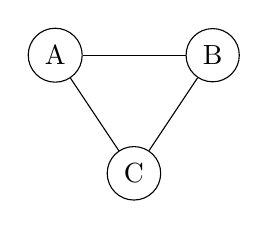
\begin{tikzpicture}
                \node[circle,draw] (A) at (0,0) {A};
                \node[circle,draw] (B) at (2,0) {B};
                \node[circle,draw] (C) at (1,-1.5) {C};
                \draw (A) -- (B);
                \draw (B) -- (C);
                \draw (C) -- (A);
            \end{tikzpicture}
            \caption{An example graph.}
        \end{figure}
% draw graph using latex
        \column{0.5\textwidth}
        \begin{itemize}
            \item Nodes (Vertices)
            \item Edges
            \item Directed vs. Undirected
            \item Weighted vs. Unweighted
        \end{itemize}
    \end{columns}
\end{frame}

\begin{frame}{Graph Illustration with \LaTeX}
    \begin{figure}
        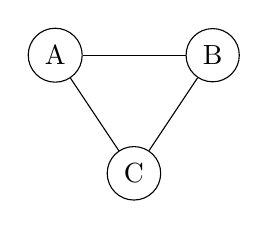
\begin{tikzpicture}
            \node[circle,draw] (A) at (0,0) {A};
            \node[circle,draw] (B) at (2,0) {B};
            \node[circle,draw] (C) at (1,-1.5) {C};
            \draw (A) -- (B);
            \draw (B) -- (C);
            \draw (C) -- (A);
        \end{tikzpicture}
        \caption{A simple graph created with \LaTeX{} and \texttt{tikz}.}
    \end{figure}
\end{frame}

\begin{frame}{Directed vs. Undirected Graphs}
    \begin{columns}
        \column{0.5\textwidth}
        \begin{figure}
            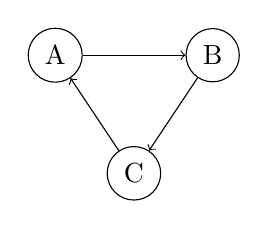
\begin{tikzpicture}
                \node[circle,draw] (A) at (0,0) {A};
                \node[circle,draw] (B) at (2,0) {B};
                \node[circle,draw] (C) at (1,-1.5) {C};
                \draw[->] (A) -- (B);
                \draw[->] (B) -- (C);
                \draw[->] (C) -- (A);
            \end{tikzpicture}
            \caption{Directed graph.}
        \end{figure}

        \column{0.5\textwidth}
        \begin{figure}
            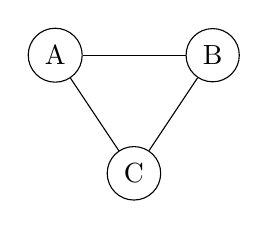
\begin{tikzpicture}
                \node[circle,draw] (A) at (0,0) {A};
                \node[circle,draw] (B) at (2,0) {B};
                \node[circle,draw] (C) at (1,-1.5) {C};
                \draw (A) -- (B);
                \draw (B) -- (C);
                \draw (C) -- (A);
            \end{tikzpicture}
            \caption{Undirected graph.}
        \end{figure}
    \end{columns}
\end{frame}

\begin{frame}{Weighted Graphs}
    \begin{columns}
        \column{0.5\textwidth}
        \begin{figure}
            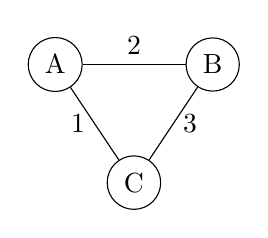
\begin{tikzpicture}
                \node[circle,draw] (A) at (0,0) {A};
                \node[circle,draw] (B) at (2,0) {B};
                \node[circle,draw] (C) at (1,-1.5) {C};
                \draw (A) -- node[above] {2} (B);
                \draw (B) -- node[right] {3} (C);
                \draw (C) -- node[left] {1} (A);
            \end{tikzpicture}
            \caption{Weighted graph.}
        \end{figure}

        \column{0.5\textwidth}
        \begin{itemize}
            \item Edges have associated weights.
            \item Reflects the cost or distance between nodes.
        \end{itemize}
    \end{columns}
\end{frame}

\begin{frame}{Graph Algorithms - BFS and DFS}
    \begin{columns}
        \column{0.5\textwidth}
        \begin{figure}
            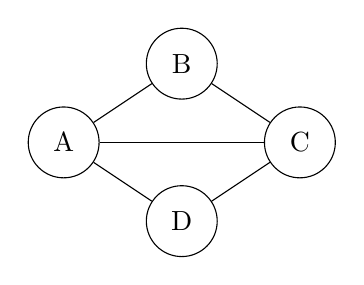
\begin{tikzpicture}[every node/.style={circle, draw, minimum size=9mm}]
                \node (A) at (0,0) {A};
                \node (B) at (1.5,1) {B};
                \node (C) at (3,0) {C};
                \node (D) at (1.5,-1) {D};
                \draw (A) -- (B) -- (C) -- (D) -- (A);
                \draw (A) -- (C);
            \end{tikzpicture}
            \caption{Example graph for BFS and DFS.}
        \end{figure}

        \column{0.5\textwidth}
        \begin{itemize}
            \item \textbf{BFS (Breadth-First Search):}
            \begin{itemize}
                \item Start from the source node (A).
                \item Visit neighbors before moving to the next level.
            \end{itemize}
            \item \textbf{DFS (Depth-First Search):}
            \begin{itemize}
                \item Start from the source node (A).
                \item Explore as far as possible before backtracking.
            \end{itemize}
        \end{itemize}
    \end{columns}
\end{frame}

\begin{frame}{BFS and DFS - Example}
    \begin{columns}
        \column{0.5\textwidth}
        \begin{figure}
            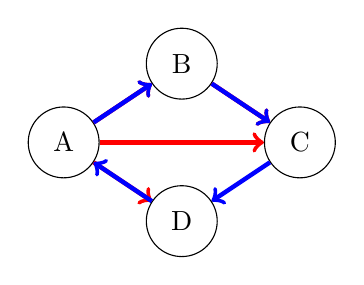
\begin{tikzpicture}[every node/.style={circle, draw, minimum size=9mm}]
                \node (A) at (0,0) {A};
                \node (B) at (1.5,1) {B};
                \node (C) at (3,0) {C};
                \node (D) at (1.5,-1) {D};
                \draw (A) -- (B) -- (C) -- (D) -- (A);
                \draw (A) -- (C);
                
                % BFS
                \draw[ultra thick, red, ->] (A) -- (B);
                \draw[ultra thick, red, ->] (A) -- (C);
                \draw[ultra thick, red, ->] (A) -- (D);
                \draw[ultra thick, red, ->] (B) -- (C);
                
                % DFS
                \draw[ultra thick, blue, ->] (A) -- (B);
                \draw[ultra thick, blue, ->] (B) -- (C);
                \draw[ultra thick, blue, ->] (C) -- (D);
                \draw[ultra thick, blue, ->] (D) -- (A);
            \end{tikzpicture}
            \caption{BFS and DFS on the example graph.}
        \end{figure}

        \column{0.5\textwidth}
        \begin{itemize}
            \item \textbf{BFS (Breadth-First Search):}
            \begin{itemize}
                \item Start from the source node (A).
                \item Visit neighbors before moving to the next level.
            \end{itemize}
            \item \textbf{DFS (Depth-First Search):}
            \begin{itemize}
                \item Start from the source node (A).
                \item Explore as far as possible before backtracking.
            \end{itemize}
        \end{itemize}
    \end{columns}
\end{frame}

\begin{frame}{Common Graph Algorithms}
    \begin{itemize}
        \item Breadth-First Search (BFS)
        \item Depth-First Search (DFS)
        \item Dijkstra's Algorithm
        \item Kruskal's Algorithm
        \item Eulerian and Hamiltonian Paths
    \end{itemize}
\end{frame}

\begin{frame}{Graphs in \LaTeX{} - Advanced}
    \begin{itemize}
        \item \texttt{tikz} package allows advanced customization.
        \item Create complex graphs with precise control.
        \item Ideal for academic and technical presentations.
    \end{itemize}
\end{frame}

\begin{frame}{Conclusion}
    \begin{itemize}
        \item Graph theory is a powerful tool with diverse applications.
        \item \LaTeX{} provides an efficient way to create high-quality presentations.
        \item Experiment with \texttt{tikz} for more advanced graph representations.
        \item Thank you for your attention!
    \end{itemize}
\end{frame}

\end{document}